{\LARGE Output:}

Again, is the magnitude of X nonzero for the expected frequenies? Is the phase of X correct?

Yes, It matched the expectations I Stated from previous(part C)

\begin{figure}[!htbp]
  \centering
    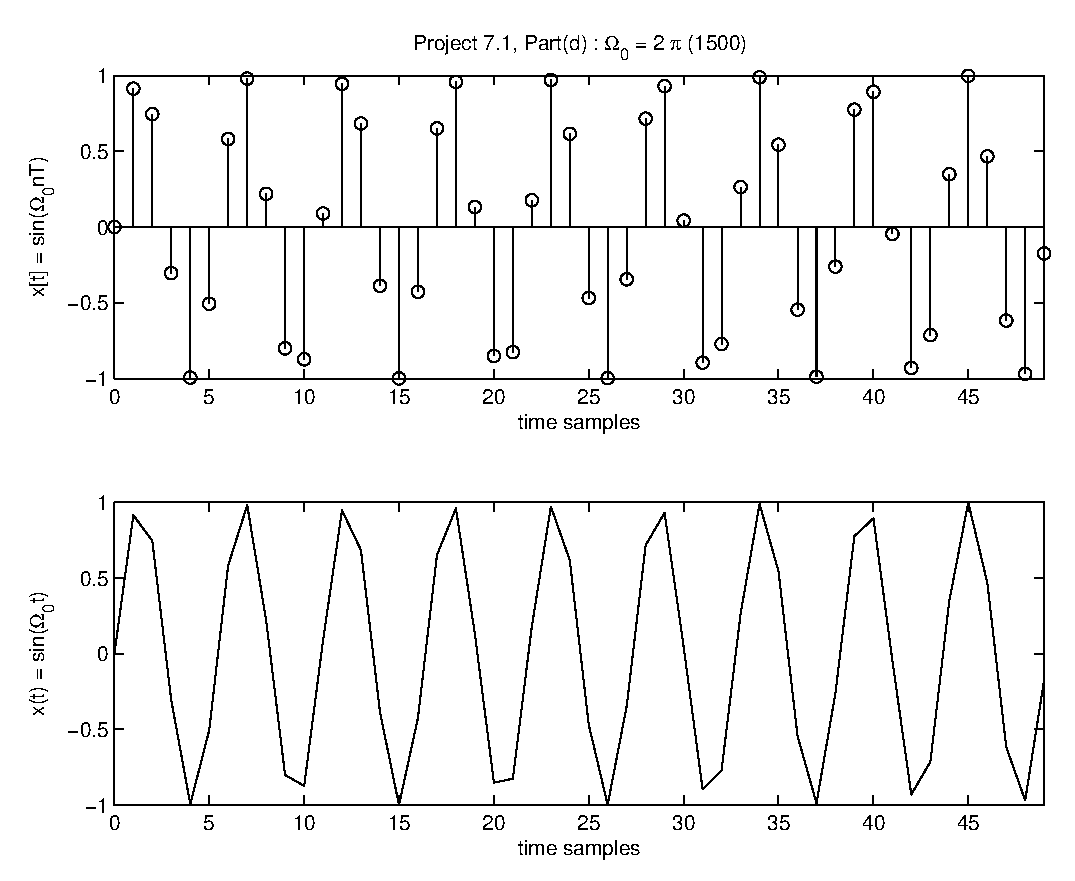
\includegraphics[width=0.7\textwidth]{Part1/Output/Figures/proj71PartD1.eps}
  \caption{Output for 7.1 Part D |Part B for $\Omega_0 = 2\pi(1500)$ }
\end{figure}

\begin{figure}[!htbp]
  \centering
    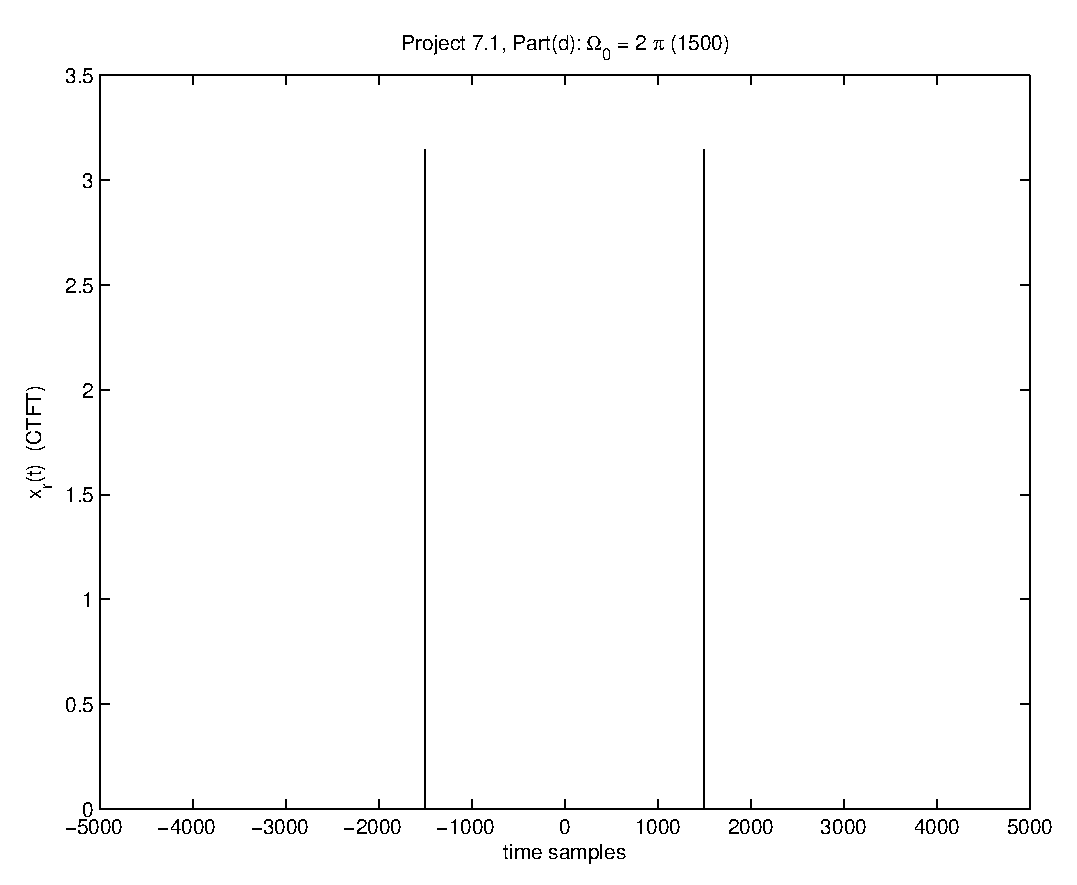
\includegraphics[width=0.7\textwidth]{Part1/Output/Figures/proj71PartD2.eps}
  \caption{Output for 7.1 Part D |Part C for $\Omega_0 = 2\pi(1500)$ }
\end{figure}

\begin{figure}[!htbp]
  \centering
    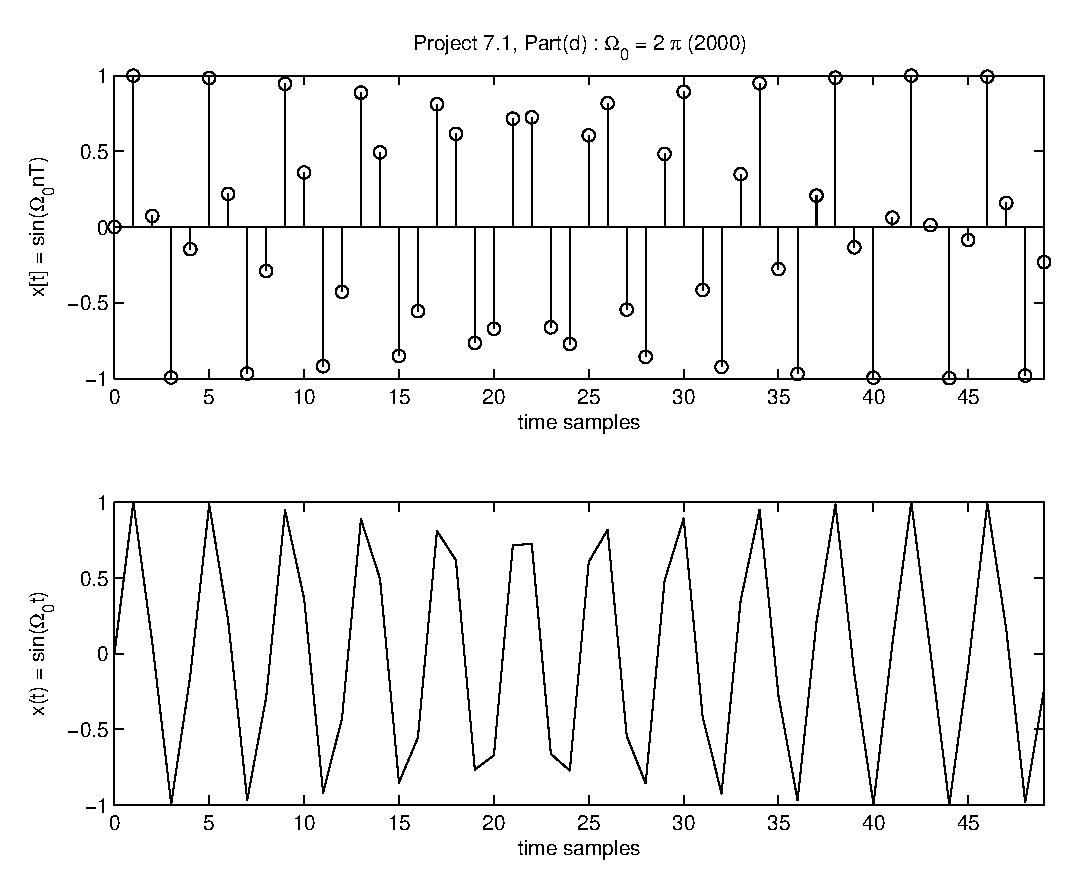
\includegraphics[width=0.7\textwidth]{Part1/Output/Figures/proj71PartD3.eps}
  \caption{Output for 7.1 Part D |Part B for $\Omega_0 = 2\pi(2000)$ }
\end{figure}

\begin{figure}[!htbp]
  \centering
    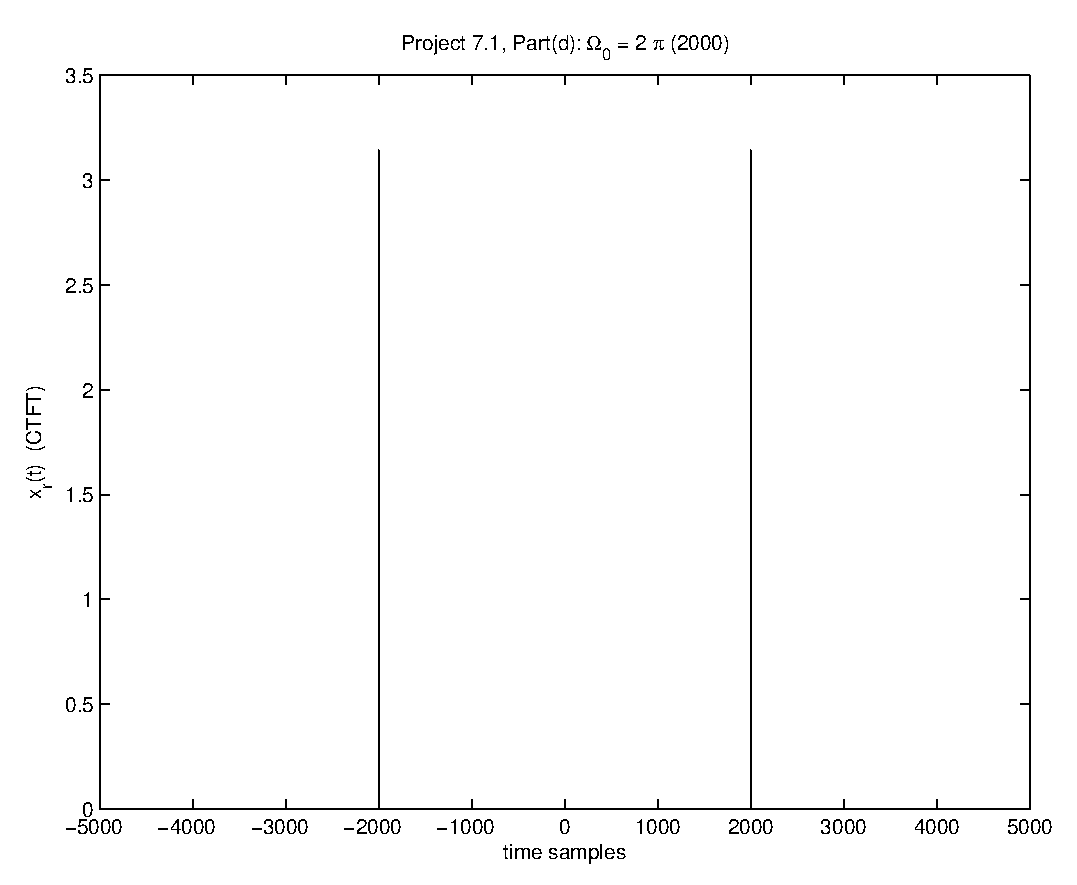
\includegraphics[width=0.7\textwidth]{Part1/Output/Figures/proj71PartD4.eps}
  \caption{Output for 7.1 Part D |Part C for $\Omega_0 = 2\pi(2000)$ }
\end{figure}

\pagebreak
